
\chapter{Proposed Methodology}
\label{chap:methodology}

\section{Problem Formulation}

The thesis addresses supervised neural decoding in the perception setting. Each training example consists of a pair $(x_i, z_i)$, where $x_i$ is the preprocessed fMRI feature vector and $z_i$ is a target image representation extracted from the corresponding viewed stimulus. The learning objective is to estimate a decoder $f_{\theta}$ such that the predicted representation
\begin{equation}
\hat{z}_i = f_{\theta}(x_i)
\label{eq:decoder_prediction}
\end{equation}
is close to the correct target and sufficiently discriminative relative to all other targets in the gallery.

In practice, the decoder does not solve a single homogeneous problem. The later stages of the thesis distinguish between three complementary roles: compact retrieval, reranking, and rich regression. This leads naturally to a multi-head architecture,
\begin{equation}
\big(\hat{z}^{(c)}_i, \hat{z}^{(r)}_i, \hat{z}^{(g)}_i\big) = f_{\theta}(x_i),
\label{eq:multihead_decoder}
\end{equation}
where the superscripts denote the compact head, rerank head, and rich generative/regression head, respectively.

\section{Data Preparation and Preprocessing}

The preprocessing pipeline transforms raw NSD-derived activity into model-ready vectors. The core steps are voxel selection, repeated-trial aggregation when needed, subject/session indexing, per-session normalization, and alignment with image identifiers and cached visual targets. A crucial principle throughout the project is that train/validation separation must occur at the image level, not merely at the trial level, so that repeated observations of the same image do not leak across splits \cite{Allen2022}.

If $x_{i,s}$ denotes the feature vector for sample $i$ in session $s$, z-scoring is performed using statistics estimated only from the training data of that session:
\begin{equation}
\tilde{x}_{i,s} = \frac{x_{i,s} - \mu_s^{\mathrm{train}}}{\sigma_s^{\mathrm{train}} + \varepsilon}.
\label{eq:zscore}
\end{equation}
This reduces session-specific drift while preserving discriminative variation relevant to decoding. In practical terms, the preprocessing stage is not a mere data-cleaning step; it is part of the scientific method, because even a strong architecture becomes meaningless if the split logic or target lookup is incorrect.

\begin{figure}[htbp]
    \centering
    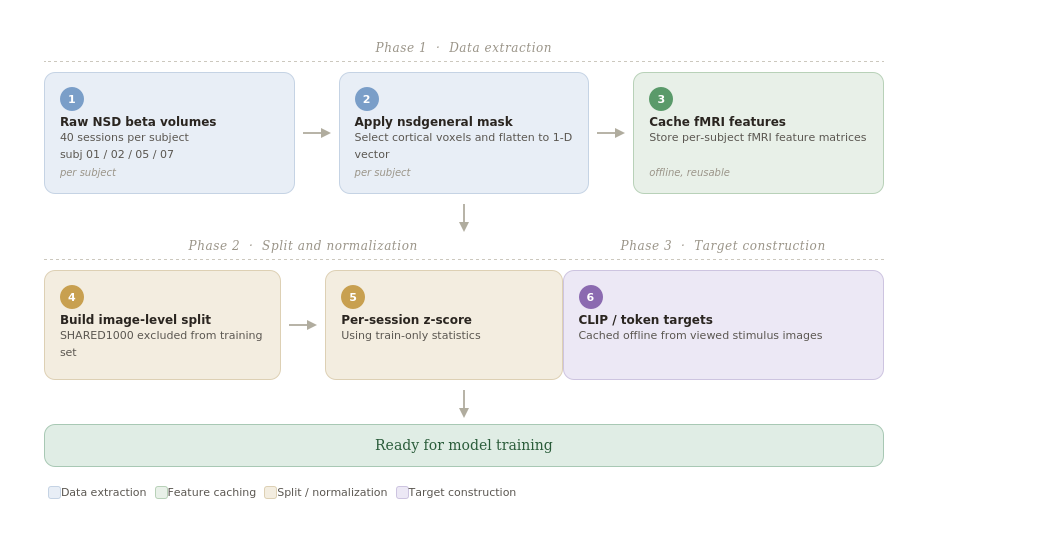
\includegraphics[width=\textwidth]{preprocessing_pipeline.png}
    \caption{Preprocessing and target-construction workflow used in the thesis. The pipeline emphasizes offline caching, image-level split integrity, and per-session normalization before model training.}
    \label{fig:preprocessing_pipeline}
\end{figure}

\section{Latent Targets}

The primary targets are CLIP image embeddings or derived token-level variants obtained from the viewed stimulus image. Let $\phi(I_i)$ denote the target representation extracted from image $I_i$ by a pretrained visual model. The simplest pooled-target formulation uses
\begin{equation}
 z_i = \phi(I_i) \in \mathbb{R}^{d},
\label{eq:target_embedding}
\end{equation}
while richer variants preserve token-level or multi-scale structure. The experiments reported in the thesis show that target quality and granularity have a large effect on retrieval performance, especially when the decoder is strong enough to exploit that additional information \cite{Radford2021,Scotti2023}.

In the methodological evolution of the project, target design became one of the decisive axes of improvement. Compact pooled targets are easier to optimize for shortlist retrieval, whereas richer targets preserve more semantic and structural information for downstream regression and generative reconstruction. The final system therefore treats target richness as a design choice rather than as a universally monotone improvement.

\section{Training Objectives}

The compact head is primarily optimized for ranking. A standard contrastive formulation is the InfoNCE loss \cite{Oord2018}:
\begin{equation}
\mathcal{L}_{\mathrm{NCE}} = -\frac{1}{N}\sum_{i=1}^{N}
\log
\frac{\exp\left(\cos(\hat{z}^{(c)}_i, z_i)/\tau\right)}
{\sum_{j=1}^{N} \exp\left(\cos(\hat{z}^{(c)}_i, z_j)/\tau\right)}.
\label{eq:info_nce}
\end{equation}
Here $\tau > 0$ is a temperature hyperparameter controlling the sharpness of the ranking distribution.

Some experiments model the predicted latent direction probabilistically through a von Mises--Fisher (vMF) output, a natural choice for unit-norm directional embeddings \cite{Banerjee2005}. If $\mu_i$ is a unit-norm mean direction and $\kappa_i$ is a concentration parameter, the density of the target direction can be written as
\begin{equation}
p(z_i \mid x_i) = C_d(\kappa_i)\exp\left(\kappa_i \, \mu_i^{\top} z_i\right),
\label{eq:vmf_density}
\end{equation}
where $C_d(\kappa_i)$ is the normalization constant on the unit hypersphere. This formulation is attractive because cosine geometry and directional uncertainty are naturally aligned; however, the thesis also shows that vMF training is sensitive to numerical pathologies if temperature and regularization are not tuned carefully.

The rich head is optimized with a regression-style objective that encourages absolute fidelity in latent space:
\begin{equation}
\mathcal{L}_{\mathrm{reg}} = \frac{1}{N}\sum_{i=1}^{N}\left\lVert \hat{z}^{(g)}_i - z_i \right\rVert_2^2.
\label{eq:regression_loss}
\end{equation}
The overall training objective combines multiple terms:
\begin{equation}
\mathcal{L}_{\mathrm{total}} = \lambda_c \mathcal{L}_{\mathrm{compact}} + \lambda_r \mathcal{L}_{\mathrm{rerank}} + \lambda_g \mathcal{L}_{\mathrm{reg}},
\label{eq:total_loss}
\end{equation}
where the $\lambda$ coefficients control the relative importance of the different heads.

\section{Architecture Evolution}
\label{sec:architecture_evolution}

The methodological evolution of the thesis begins with wide multilayer perceptron decoders operating on the full voxel vector. These models are intentionally simple and serve as strong baselines. Later iterations introduce probabilistic directional heads, ROI-aware tokenization, transformer-based components inspired by token processing in modern vision models \cite{Dosovitskiy2021}, and finally multi-head retrieval architectures.

The final trainable architecture described in this thesis is the V30/V35 family, which separates the decoding problem into three subproblems:
\begin{itemize}
    \item the \textbf{compact head}, which is optimised for shortlist retrieval in a stable low-dimensional space;
    \item the \textbf{rerank head}, which operates only on shortlist candidates and performs shortlist-local discrimination;
    \item the \textbf{rich head}, which preserves a higher-capacity representation useful for regression and reconstruction-oriented supervision.
\end{itemize}
This separation is one of the central design insights of the project: a single latent space is not forced to satisfy all design requirements simultaneously. The decomposition is preserved by the final exported system, which keeps the multi-head decoder trained as in V35 but replaces the two-expert milestone fusion with the inference-time cross-architecture triple score fusion described in Section~\ref{chap:experiments}.

\begin{figure}[htbp]
    \centering
    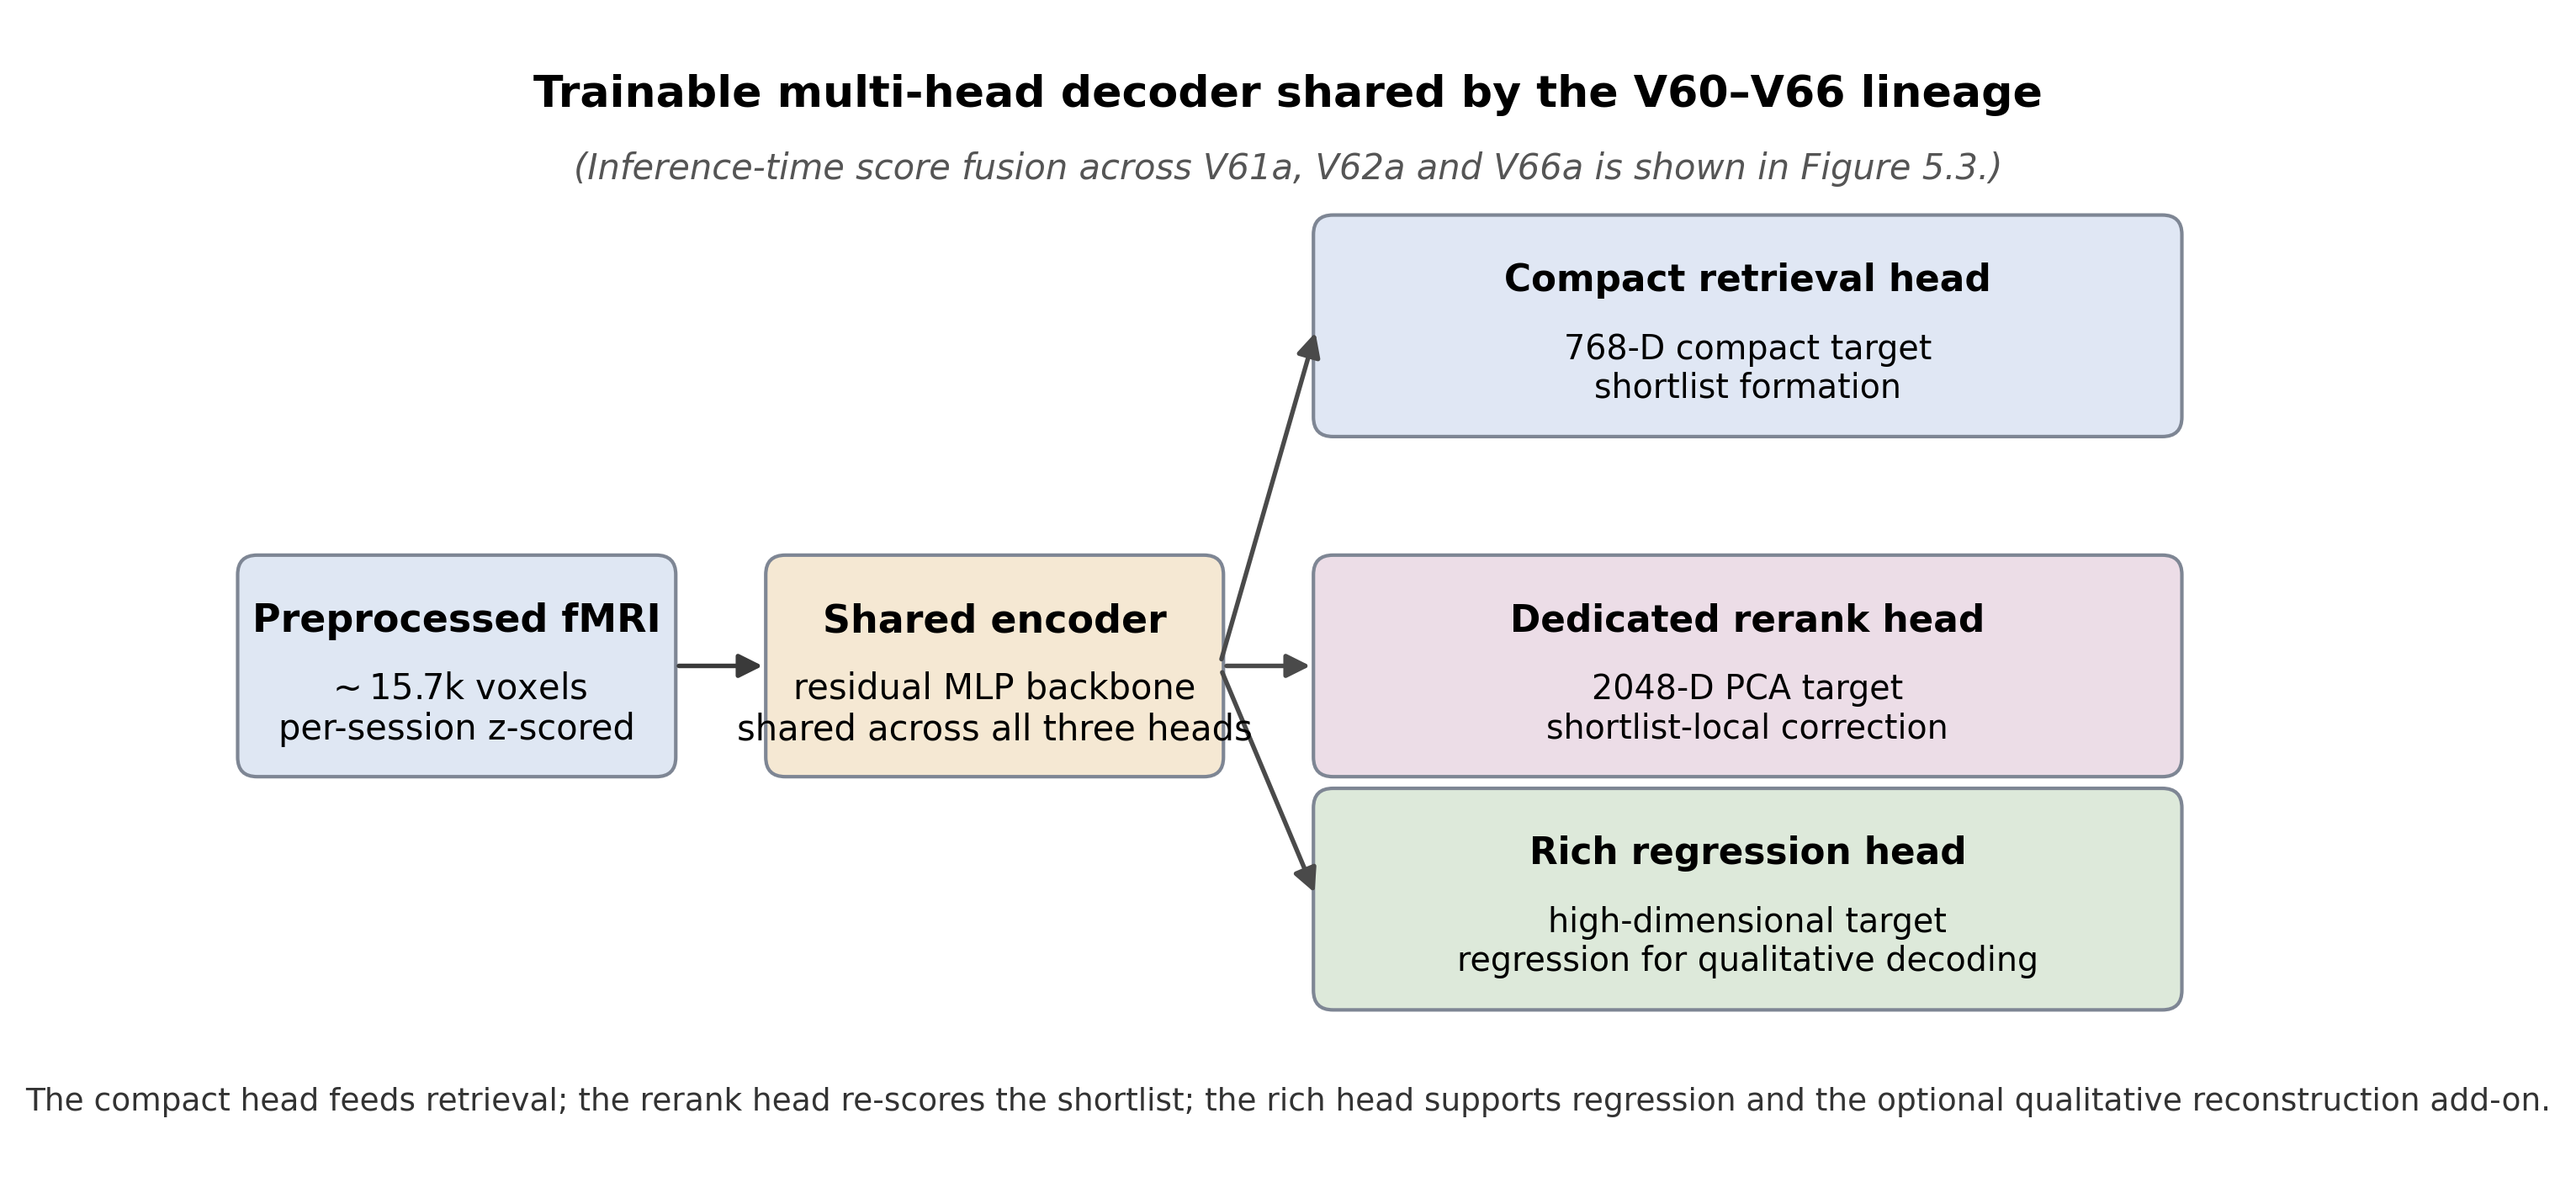
\includegraphics[width=\textwidth]{model_architecture.png}
    \caption{Trainable multi-head decoder shared by the V60--V66 lineage. A residual MLP encoder operates on the preprocessed voxel vector and feeds three task-specific heads (compact for shortlist, rerank for shortlist-local correction, rich for regression-style targets and qualitative decoding). This is the trainable architecture; the inference-time score fusion across V61a, V62a, and V66a that yields the headline SHARED1000 result is described in Section~\ref{chap:experiments} and depicted separately in Figure~\ref{fig:triple_fusion_architecture}.}
    \label{fig:model_architecture}
\end{figure}

\section{Inference and Score Fusion}

At inference time, the compact head first retrieves a shortlist of candidate images. Let $\mathcal{S}_K(x_i)$ denote the top-$K$ shortlist obtained from compact retrieval. In the earlier V30/V32 wave, the rerank head rescales those candidates locally. If $s_c(i,j)$ is the compact score and $s_r(i,j)$ is the rerank score for candidate $j$ in the shortlist of sample $i$, the shortlist-local fused score can be written as
\begin{equation}
s_{\mathrm{fusion}}(i,j) = \alpha \, s_c(i,j) + (1-\alpha) \, s_r(i,j), \qquad j \in \mathcal{S}_K(x_i),
\label{eq:fusion_score}
\end{equation}
where $\alpha \in [0,1]$ is a fusion weight. This formulation established the key methodological lesson of the thesis: reranking is most effective as a corrective signal applied inside a strong shortlist.

A first frozen fixed-fusion system extends this idea with a complementary legacy expert. Using z-score-normalized expert scores, the corresponding score combination can be written as
\begin{equation}
s_{\mathrm{milestone}}(i,j) = 0.3\,\widetilde{s}_{c,\mathrm{CSLS}}(i,j) + 0.7\,\widetilde{s}_{\ell,\mathrm{CSLS}}(i,j),
\label{eq:best_fusion_score}
\end{equation}
with $\widetilde{s}_{c,\mathrm{CSLS}}$ denoting the normalized compact-CSLS score from V35 and $\widetilde{s}_{\ell,\mathrm{CSLS}}$ denoting the normalized legacy-CSLS score from N1v28a. The rerank branch remains methodologically important and still informs the architecture; the V35 plus legacy combination is retained as a milestone result that validates the compact--rerank--rich decomposition under expert fusion.

After validating this compact, rerank, and rich decomposition, the final inference-time extension explored stronger token-space decoding and cross-architecture score fusion. The exported best system replaces the two-expert fusion above with a frozen score-level combination of three retrieval experts that span different target spaces and different inductive biases: a 197K token-space model (V61a) evaluated with 16-draw Monte Carlo test-time augmentation (MC-TTA-16), a 768-D CLS retrieval model (V62a), and a 768-D ROI-pretrained model (V66a). With $\widetilde{s}_{1,\mathrm{CSLS}}$, $\widetilde{s}_{2,\mathrm{CSLS}}$, and $\widetilde{s}_{3,\mathrm{CSLS}}$ denoting the normalized CSLS scores of these three experts, the final retrieval score is
\begin{equation}
s_{\mathrm{final}}(i,j) = 0.7\,\widetilde{s}_{1,\mathrm{CSLS}}(i,j) + 0.1\,\widetilde{s}_{2,\mathrm{CSLS}}(i,j) + 0.2\,\widetilde{s}_{3,\mathrm{CSLS}}(i,j),
\label{eq:triple_fusion_score}
\end{equation}
evaluated with CSLS neighbourhood size $k=3$. The weights, the CSLS neighbourhood size, and the choice of experts are all frozen before SHARED1000 evaluation, so the final system performs no test-time tuning. The final fusion is applied only at the retrieval-score level: it combines normalised CSLS score matrices from \emph{independently trained} retrieval experts and does not define a single fused latent representation. Equation~\eqref{eq:triple_fusion_score} is therefore not an end-to-end jointly trained fusion architecture and shares no decoder weights between the three experts; the trainable multi-head decomposition described in Section~\ref{sec:architecture_evolution} and depicted in Figure~\ref{fig:model_architecture} characterises the V30/V35 family, while V61a, V62a, and V66a are separate fine-tuned models whose only point of interaction is Equation~\eqref{eq:triple_fusion_score}.

A useful way to interpret the overall design is therefore that the first stage solves a difficult global search problem, the rerank branch provides shortlist-local discrimination, the two-expert milestone fusion validates that complementary experts can be combined at inference time, and the final triple fusion combines partially different information from three target spaces and architecture families through frozen score-level weights, without retraining the backbone. This division of labour is one of the main methodological lessons of the project.

\section{Reproducibility Principles}

A significant part of the methodology is dedicated to reproducibility. The project maintains versioned experiment configurations, cached targets, explicit split logic, and a strict separation between training-time and evaluation-time computations. This is especially important in a thesis context because the scientific value of the results depends not only on the final metric values, but also on the ability to explain why those values were obtained and how they changed across experimental waves.

The practical implication is that every experiment is treated as a traceable artifact with explicit inputs, outputs, and evaluation scripts. In a research area where silent alignment bugs can invalidate an otherwise sophisticated system, reproducibility is not just a software-engineering virtue; it is a core scientific requirement.
